\documentclass[journal,12pt,twocolumn]{IEEEtran}

\usepackage{setspace}
\usepackage{gensymb}

\singlespacing


\usepackage[cmex10]{amsmath}

\usepackage{amsthm}

\usepackage{mathrsfs}
\usepackage{txfonts}
\usepackage{stfloats}
\usepackage{bm}
\usepackage{cite}
\usepackage{cases}
\usepackage{subfig}

\usepackage{longtable}
\usepackage{multirow}

\usepackage{enumitem}
\usepackage{mathtools}
\usepackage{steinmetz}
\usepackage{tikz}
\usepackage{circuitikz}
\usepackage{verbatim}
\usepackage{tfrupee}
\usepackage[breaklinks=true]{hyperref}
\usepackage{graphicx}
\usepackage{tkz-euclide}
\usepackage{float}

\usetikzlibrary{calc,math}
\usepackage{listings}
    \usepackage{color}                                            %%
    \usepackage{array}                                            %%
    \usepackage{longtable}                                        %%
    \usepackage{calc}                                             %%
    \usepackage{multirow}                                         %%
    \usepackage{hhline}                                           %%
    \usepackage{ifthen}                                           %%
    \usepackage{lscape}     
\usepackage{multicol}
\usepackage{chngcntr}

\DeclareMathOperator*{\Res}{Res}

\renewcommand\thesection{\arabic{section}}
\renewcommand\thesubsection{\thesection.\arabic{subsection}}
\renewcommand\thesubsubsection{\thesubsection.\arabic{subsubsection}}

\renewcommand\thesectiondis{\arabic{section}}
\renewcommand\thesubsectiondis{\thesectiondis.\arabic{subsection}}
\renewcommand\thesubsubsectiondis{\thesubsectiondis.\arabic{subsubsection}}


\hyphenation{op-tical net-works semi-conduc-tor}
\def\inputGnumericTable{}                                 %%

\lstset{
%language=C,
frame=single, 
breaklines=true,
columns=fullflexible
}
\begin{document}
\newtheorem{theorem}{Theorem}[section]
\newtheorem{problem}{Problem}
\newtheorem{proposition}{Proposition}[section]
\newtheorem{lemma}{Lemma}[section]
\newtheorem{corollary}[theorem]{Corollary}
\newtheorem{example}{Example}[section]
\newtheorem{definition}[problem]{Definition}

\newcommand{\BEQA}{\begin{eqnarray}}
\newcommand{\EEQA}{\end{eqnarray}}
\newcommand{\define}{\stackrel{\triangle}{=}}
\bibliographystyle{IEEEtran}
\providecommand{\mbf}{\mathbf}
\providecommand{\pr}[1]{\ensuremath{\Pr\left(#1\right)}}
\providecommand{\qfunc}[1]{\ensuremath{Q\left(#1\right)}}
\providecommand{\sbrak}[1]{\ensuremath{{}\left[#1\right]}}
\providecommand{\lsbrak}[1]{\ensuremath{{}\left[#1\right.}}
\providecommand{\rsbrak}[1]{\ensuremath{{}\left.#1\right]}}
\providecommand{\brak}[1]{\ensuremath{\left(#1\right)}}
\providecommand{\lbrak}[1]{\ensuremath{\left(#1\right.}}
\providecommand{\rbrak}[1]{\ensuremath{\left.#1\right)}}
\providecommand{\cbrak}[1]{\ensuremath{\left\{#1\right\}}}
\providecommand{\lcbrak}[1]{\ensuremath{\left\{#1\right.}}
\providecommand{\rcbrak}[1]{\ensuremath{\left.#1\right\}}}
\theoremstyle{remark}
\newtheorem{rem}{Remark}
\newcommand{\sgn}{\mathop{\mathrm{sgn}}}
\providecommand{\abs}[1]{\vert#1\vert}
\providecommand{\res}[1]{\Res\displaylimits_{#1}} 
\providecommand{\norm}[1]{\lVert#1\rVert}
%\providecommand{\norm}[1]{\lVert#1\rVert}
\providecommand{\mtx}[1]{\mathbf{#1}}
\providecommand{\mean}[1]{E[ #1 ]}
\providecommand{\fourier}{\overset{\mathcal{F}}{ \rightleftharpoons}}
%\providecommand{\hilbert}{\overset{\mathcal{H}}{ \rightleftharpoons}}
\providecommand{\system}{\overset{\mathcal{H}}{ \longleftrightarrow}}
	%\newcommand{\solution}[2]{\textbf{Solution:}{#1}}
\newcommand{\solution}{\noindent \textbf{Solution: }}
\newcommand{\cosec}{\,\text{cosec}\,}
\providecommand{\dec}[2]{\ensuremath{\overset{#1}{\underset{#2}{\gtrless}}}}
\newcommand{\myvec}[1]{\ensuremath{\begin{pmatrix}#1\end{pmatrix}}}
\newcommand{\mydet}[1]{\ensuremath{\begin{vmatrix}#1\end{vmatrix}}}
\numberwithin{equation}{subsection}
\makeatletter
\@addtoreset{figure}{problem}
\makeatother
\let\StandardTheFigure\thefigure
\let\vec\mathbf
\renewcommand{\thefigure}{\theproblem}
\def\putbox#1#2#3{\makebox[0in][l]{\makebox[#1][l]{}\raisebox{\baselineskip}[0in][0in]{\raisebox{#2}[0in][0in]{#3}}}}
     \def\rightbox#1{\makebox[0in][r]{#1}}
     \def\centbox#1{\makebox[0in]{#1}}
     \def\topbox#1{\raisebox{-\baselineskip}[0in][0in]{#1}}
     \def\midbox#1{\raisebox{-0.5\baselineskip}[0in][0in]{#1}}
\vspace{3cm}
\title{Quiz 2}
\author{Haritha R \\ AI20BTECH11010}
\maketitle
\newpage
\bigskip
\renewcommand{\thefigure}{\theenumi}
\renewcommand{\thetable}{\theenumi}
Download python codes from
%
\begin{lstlisting}
https://github.com/harithar1234/EE3900-Haritha/tree/main/quiz2/code
\end{lstlisting}
%

\section*{QUESTION}
\textbf{The z-transform/3.3(b)}
\begin{enumerate}
Determine the z-transform of each of the following sequences. Include with your answer the region of convergence in the z-plane and a sketch of the pole-zero plot. Express all sums in closed form.

\begin{equation*}
(b) x_b[n]=
\begin{cases}
      1, & \text{0 $\leq$ n $\leq$ N-1}\\
      0, & \text{otherwise}
    \end{cases}       
\end{equation*}

\section*{SOLUTION}
The z-transform of a sequence x[n] is defined as
\begin{align}
   X(z) = \sum_{n= -\infty}^{\infty} x[n] z^{-n} 
\end{align}
The z-transform of the sequence $x_b [n] $ is:
\begin{align}
   X_b(z) = \sum_{n= -\infty}^{\infty} x_b[n] z^{-n} 
\end{align}
since the sequence $x_b [n] $ is non-zero only for \\
0 $\leq$ n $\leq$ N-1, The z-transform of the sequence $x_b [n] $ is:
\begin{align}
X_b(z) = \sum_{n=0}^{N-1} x_b[n] z^{-n} \\
X_b(z) = \sum_{n=0}^{N-1} z^{-n} \\
X_b(z)= \frac{1-(z^{-N})}{1-(z^{-1})} = \frac{1}{z^{N-1}}\frac{z^N-1}{z-1}
\end{align}
The region of convergence, known as the ROC for a given  $x_b[n]$, is defined as the range of  z  for which the z-transform converges.The condition to be satisfied for convergence is:
\begin{align}
    \sum_{n=-\infty}^{\infty} \abs{x_b[n] z^{-n} } < \infty\\
     \sum_{n=0}^{N-1} \abs{x_b[n] z^{-n} } < \infty\\
     \sum_{n=0}^{N-1} \abs{ z^{-n} } < \infty
\end{align}
the sum $\sum_{n=0}^{N-1} \abs{ z^{-n} }$ will finite as $z^{-1}$ is finite, which requires $z\neq 0$. The ROC of $X_b(z)$ includes the entire z-plane, with the exception of origin.
\begin{align*}
   \text{ ROC of } X_b(z): \abs{z}>0 
\end{align*}
\begin{align}
 X_b(z)= \frac{1-(z^{-N})}{1-(z^{-1})}   
\end{align}
The zeros of $X_b(z)$ will be the solutions of the equation $z^N=1$.\\The zeros of $X_b(z)$ will vary depending on N. $(N \geq 2)$.however z=1 will always be zero irrespective of N.
The pole of $X_b(z)$ is z=1 always.

\begin{figure}[h]
    {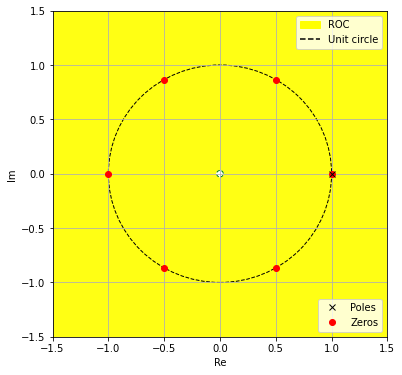
\includegraphics{plot.png}}
    \caption{\Large{Plot of zeros for N=6,plot of poles and region of convergence }}
\end{figure}
\end{enumerate}
\end{document}
